\documentclass[a4paper]{article}

\usepackage[spanish]{babel} % Le indicamos a LaTeX que vamos a escribir en espa�ol.
\usepackage[latin1]{inputenc} % Permite utilizar tildes y e�es normalmente
\usepackage{pdfpages}
\usepackage{listings}
\usepackage{xcolor}
\setlength{\parindent}{0cm}
\lstset { %
    language=C++,
    backgroundcolor=\color{black!10}, % set backgroundcolor
    basicstyle=\footnotesize,% basic font setting
    linewidth=\textwidth{},
    showstringspaces=false,
    breakatwhitespace=true,
    breaklines=true 
}

\usepackage{ifthen}
\usepackage{amssymb}
\usepackage{multicol}
\usepackage{graphicx}
\usepackage[absolute]{textpos}
\makeatletter

\@ifclassloaded{beamer}{%
  \newcommand{\tocarEspacios}{%
    \addtolength{\leftskip}{4em}%
    \addtolength{\parindent}{-3em}%
  }%
}
{%
  \usepackage[top=1cm,bottom=2cm,left=1cm,right=1cm]{geometry}%
  \usepackage{color}%
  \newcommand{\tocarEspacios}{%
    \addtolength{\leftskip}{5em}%
    \addtolength{\parindent}{-3em}%
  }%
}

\newcommand{\encabezadoDeProblema}[4]{%
  % Ponemos la palabrita problema en tt
%  \noindent%
  {\normalfont\bfseries\ttfamily problema}%
  % Ponemos el nombre del problema
  \ %
  {\normalfont\ttfamily #2}%
  \ 
  % Ponemos los parametros
  (#3)%
  \ifthenelse{\equal{#4}{}}{}{%
  \ =\ %
  % Ponemos el nombre del resultado
  {\normalfont\ttfamily #1}%
  % Por ultimo, va el tipo del resultado
  \ : #4}
}

\newcommand{\encabezadoDeTipo}[2]{%
  % Ponemos la palabrita tipo en tt
  {\normalfont\bfseries\ttfamily tipo}%
  % Ponemos el nombre del tipo
  \ %
  {\normalfont\ttfamily #2}%
  \ifthenelse{\equal{#1}{}}{}{$\langle$#1$\rangle$}
}

% Primero definiciones de cosas al estilo title, author, date

\def\materia#1{\gdef\@materia{#1}}
\def\@materia{No especifi\'o la materia}
\def\lamateria{\@materia}

\def\cuatrimestre#1{\gdef\@cuatrimestre{#1}}
\def\@cuatrimestre{No especifi\'o el cuatrimestre}
\def\elcuatrimestre{\@cuatrimestre}

\def\anio#1{\gdef\@anio{#1}}
\def\@anio{No especifi\'o el anio}
\def\elanio{\@anio}

\def\fecha#1{\gdef\@fecha{#1}}
\def\@fecha{\today}
\def\lafecha{\@fecha}

\def\nombre#1{\gdef\@nombre{#1}}
\def\@nombre{No especific'o el nombre}
\def\elnombre{\@nombre}

\def\practicas#1{\gdef\@practica{#1}}
\def\@practica{No especifi\'o el n\'umero de pr\'actica}
\def\lapractica{\@practica}


% Esta macro convierte el numero de cuatrimestre a palabras
\newcommand{\cuatrimestreLindo}{
  \ifthenelse{\equal{\elcuatrimestre}{1}}
  {Primer cuatrimestre}
  {\ifthenelse{\equal{\elcuatrimestre}{2}}
  {Segundo cuatrimestre}
  {Verano}}
}


\newcommand{\depto}{{UBA -- Facultad de Ciencias Exactas y Naturales --
      Departamento de Computaci\'on}}

\newcommand{\titulopractica}{
  \centerline{\depto}
  \vspace{1ex}
  \centerline{{\Large\lamateria}}
  \vspace{0.5ex}
  \centerline{\cuatrimestreLindo de \elanio}
  \vspace{2ex}
  \centerline{{\huge Pr\'actica \lapractica -- \elnombre}}
  \vspace{5ex}
  \arreglarincisos
  \newcounter{ejercicio}
  \newenvironment{ejercicio}{\stepcounter{ejercicio}\textbf{Ejercicio
      \theejercicio}%
    \renewcommand\@currentlabel{\theejercicio}%
  }{\vspace{0.2cm}}
}  


\newcommand{\titulotp}{
  \centerline{\depto}
  \vspace{1ex}
  \centerline{{\Large\lamateria}}
  \vspace{0.5ex}
  \centerline{\cuatrimestreLindo de \elanio}
  \vspace{0.5ex}
  \centerline{\lafecha}
  \vspace{2ex}
  \centerline{{\huge\elnombre}}
  \vspace{5ex}
}


%practicas
\newcommand{\practica}[2]{%
    \title{Pr\'actica #1 \\ #2}
    \author{Algoritmos y Estructuras de Datos I}
    \date{Segundo Cuatrimestre 2015}

    \maketitlepractica{#1}{#2}
}

\newcommand \maketitlepractica[2] {%
\begin{center}
\begin{tabular}{r cr}
 \begin{tabular}{c}
{\large\bf\textsf{\ Algoritmos y Estructuras de Datos I\ }}\\ 
Segundo Cuatrimestre 2015\\
\title{\normalsize Gu\'ia Pr\'actica #1 \\ \textbf{#2}}\\
\@title
\end{tabular} &
\begin{tabular}{@{} p{1.6cm} @{}}
\includegraphics[width=1.6cm]{logodpt.jpg}
\end{tabular} &
\begin{tabular}{l @{}}
 \emph{Departamento de Computaci\'on} \\
 \emph{Facultad de Ciencias Exactas y Naturales} \\
 \emph{Universidad de Buenos Aires} \\
\end{tabular} 
\end{tabular}
\end{center}

\bigskip
}


% Simbolos varios

\newcommand{\ent}{\ensuremath{\mathbb{Z}}}
\newcommand{\float}{\ensuremath{\mathbb{R}}}
\newcommand{\bool}{\ensuremath{\mathsf{Bool}}}
\newcommand{\True}{\ensuremath{\mathrm{True}}}
\newcommand{\False}{\ensuremath{\mathrm{False}}}
\newcommand{\Then}{\ensuremath{\rightarrow}}
\newcommand{\Iff}{\ensuremath{\leftrightarrow}}
\newcommand{\implica}{\ensuremath{\longrightarrow}}
\newcommand{\IfThenElse}[3]{\ensuremath{\mathsf{if}\ #1\ \mathsf{then}\ #2\ \mathsf{else}\ #3}}


\newcommand{\rango}[2]{[#1\twodots#2]}
\newcommand{\comp}[2]{[\,#1\,|\,#2\,]}

\newcommand{\rangoac}[2]{(#1\twodots#2]}
\newcommand{\rangoca}[2]{[#1\twodots#2)}
\newcommand{\rangoaa}[2]{(#1\twodots#2)}

%ejercicios
\newtheorem{exercise}{Ejercicio}
\newenvironment{ejercicio}{\begin{exercise}\rm}{\end{exercise} \vspace{0.2cm}}
\newenvironment{items}{\begin{enumerate}[i)]}{\end{enumerate}}
\newenvironment{subitems}{\begin{enumerate}[a)]}{\end{enumerate}}
\newcommand{\sugerencia}[1]{\noindent \textbf{Sugerencia:} #1}

%tipos basicos
\newcommand{\rea}{\ensuremath{\mathsf{Float}}}
\newcommand{\cha}{\ensuremath{\mathsf{Char}}}

\newcommand{\mcd}{\mathrm{mcd}}
\newcommand{\prm}[1]{\ensuremath{\mathsf{prm}(#1)}}
\newcommand{\sgd}[1]{\ensuremath{\mathsf{sgd}(#1)}}

%listas
\newcommand{\TLista}[1]{[#1]}
\newcommand{\lvacia}{\ensuremath{[\ ]}}
\newcommand{\lv}{\ensuremath{[\ ]}}
\newcommand{\longitud}[1]{\left| #1 \right|}
\newcommand{\cons}[1]{\ensuremath{\mathsf{cons}}(#1)}
\newcommand{\indice}[1]{\ensuremath{\mathsf{indice}}(#1)}
\newcommand{\conc}[1]{\ensuremath{\mathsf{conc}}(#1)}
\newcommand{\cab}[1]{\ensuremath{\mathsf{cab}}(#1)}
\newcommand{\cola}[1]{\ensuremath{\mathsf{cola}}(#1)}
\newcommand{\sub}[1]{\ensuremath{\mathsf{sub}}(#1)}
\newcommand{\en}[1]{\ensuremath{\mathsf{en}}(#1)}
\newcommand{\cuenta}[2]{\mathsf{cuenta}\ensuremath{(#1, #2)}}
\newcommand{\suma}[1]{\mathsf{suma}(#1)}
\newcommand{\twodots}{\ensuremath{\mathrm{..}}}
\newcommand{\masmas}{\ensuremath{++}}

% Acumulador
\newcommand{\acum}[1]{\ensuremath{\mathsf{acum}}(#1)}
\newcommand{\acumselec}[3]{\ensuremath{\mathrm{acum}(#1 |  #2, #3)}}

% \selector{variable}{dominio}
\newcommand{\selector}[2]{#1~\ensuremath{\leftarrow}~#2}
\newcommand{\selec}{\ensuremath{\leftarrow}}


\newenvironment{problema}[4][res]{%
  % El parametro 1 (opcional) es el nombre del resultado
  % El parametro 2 es el nombre del problema
  % El parametro 3 son los parametros
  % El parametro 4 es el tipo del resultado
  % Preambulo del ambiente problema
  % Tenemos que definir los comandos requiere, asegura, modifica y aux
  \newcommand{\requiere}[2][]{%
    {\normalfont\bfseries\ttfamily requiere}%
    \ifthenelse{\equal{##1}{}}{}{\ {\normalfont\ttfamily ##1} :}\ %
    \ensuremath{##2}%
    {\normalfont\bfseries\,;\par}%
  }
  \newcommand{\asegura}[2][]{%
    {\normalfont\bfseries\ttfamily asegura}%
    \ifthenelse{\equal{##1}{}}{}{\ {\normalfont\ttfamily ##1} :}\
    \ensuremath{##2}%
    {\normalfont\bfseries\,;\par}%
  }
  \newcommand{\modifica}[1]{%
    {\normalfont\bfseries\ttfamily modifica\ }%
    \ensuremath{##1}%
    {\normalfont\bfseries\,;\par}%
  }
  \renewcommand{\aux}[4]{%
    {\normalfont\bfseries\ttfamily aux\ }%
    {\normalfont\ttfamily ##1}%
    \ifthenelse{\equal{##2}{}}{}{\ (##2)}\ : ##3\, = \ensuremath{##4}%
    {\normalfont\bfseries\,;\par}%
  }
  \newcommand{\res}{#1}
  \vspace{1ex}
  \noindent
  \encabezadoDeProblema{#1}{#2}{#3}{#4}
  % Abrimos la llave
  \{\par%
  \tocarEspacios
}
% Ahora viene el cierre del ambiente problema
{
  % Cerramos la llave
  \noindent\}
  \vspace{1ex}
}


  \newcommand{\aux}[4]{%
    {\normalfont\bfseries\ttfamily aux\ }%
    {\normalfont\ttfamily #1}%
    \ifthenelse{\equal{#2}{}}{}{\ (#2)}\ : #3\, = \ensuremath{#4}%
    {\normalfont\bfseries\,;\par}%
  }


\newcommand{\pre}[1]{\textsf{pre}\ensuremath{(#1)}}

\newcommand{\problemanom}[1]{\textsf{#1}}
\newcommand{\problemail}[3]{\textsf{problema #1}\ensuremath{(#2) = #3}}
\newcommand{\problemailsinres}[2]{\textsf{problema #1}\ensuremath{(#2)}}
\newcommand{\requiereil}[2]{\textsf{requiere #1: }\ensuremath{#2}}
\newcommand{\asegurail}[2]{\textsf{asegura #1: }\ensuremath{#2}}
\newcommand{\modificail}[1]{\textsf{modifica }\ensuremath{#1}}
\newcommand{\auxil}[2]{\textsf{aux }\ensuremath{#1 = #2}}
\newcommand{\auxilc}[4]{\textsf{aux }\ensuremath{#1( #2 ): #3 = #4}}
\newcommand{\auxnom}[1]{\textsf{aux }\ensuremath{#1}}

\newcommand{\comentario}[1]{{/*\ #1\ */}}

\newcommand{\nom}[1]{\ensuremath{\mathsf{#1}}}

% -----------------
% Tipos compuestos
% -----------------

\newcommand{\Pred}[1]{\mathit{#1}}
\newcommand{\TSet}[1]{\textsf{Conjunto}\ensuremath{\langle #1 \rangle}}
\newcommand{\TSetFinito}[1]{\textsf{Conjunto}\ensuremath{\langle #1 \rangle}}
\newcommand{\TRac}{\tiponom{Racional}}
\newcommand{\TVec}{\tiponom{Vector}}
\newcommand{\Func}[1]{\mathrm{#1}}
\newcommand{\cardinal}[1]{\left| #1 \right|}


\newcommand{\sinonimo}[2]{%
  \noindent%
  {\normalfont\bfseries\ttfamily tipo\ }%
  #1\ =\ #2%
  {\normalfont\bfseries\,;\par}
}

\newcommand{\enum}[2]{%
  \noindent%
  {\normalfont\bfseries\ttfamily tipo\ }%
  #1\ =\ #2%
  {\normalfont\bfseries\,;\par}
}

%~ \newenvironment{tipo}[1]{%
    %~ \vspace{0.2cm}
    %~ \textsf{tipo #1}\ensuremath{\{}\\
    %~ \begin{tabular}[l]{p{0.02\textwidth} p{0.02\textwidth} p{0.82 \textwidth}}
%~ }{%
    %~ \end{tabular}
%~ 
    %~ \ensuremath{\}}
    %~ \vspace{0.15cm}
%~ }
%~ 

\newenvironment{tipo}[2][]{%
  % Preambulo del ambiente tipo
  % Tenemos que definir los comandos observador (con requiere) y aux
  \newcommand{\observador}[3]{%
    {\normalfont\bfseries\ttfamily observador\ }%
    {\normalfont\ttfamily ##1}%
    \ifthenelse{\equal{##2}{}}{}{\ (##2)}\ : ##3%
    {\normalfont\bfseries\,;\par}%
  }
  \newcommand{\requiere}[2][]{{%
    \addtolength{\leftskip}{3em}%
    \setlength{\parindent}{-2em}%
    {\normalfont\bfseries\ttfamily requiere}%
    \ifthenelse{\equal{##1}{}}{}{\ {\normalfont\ttfamily ##1} :}\ 
    \ensuremath{##2}%
    {\normalfont\bfseries\,;\par}}
  }
  \newcommand{\explicacion}[1]{{%
    \addtolength{\leftskip}{3em}%
    \setlength{\parindent}{-2em}%
    \par \hspace{2.3em} ##1 %
    {\par}
    }
  }
  \newcommand{\invariante}[2][]{%
    {\normalfont\bfseries\ttfamily invariante}%
    \ifthenelse{\equal{##1}{}}{}{\ {\normalfont\ttfamily ##1} :}\ 
    \ensuremath{##2}%
    {\normalfont\bfseries\,;\par}%
  }
  \renewcommand{\aux}[4]{%
    {\normalfont\bfseries\ttfamily aux\ }%
    {\normalfont\ttfamily ##1}%
    \ifthenelse{\equal{##2}{}}{}{\ (##2)}\ : ##3\, = \ensuremath{##4}%
    {\normalfont\bfseries\,;\par}%
  }
  \vspace{1ex}
  \noindent
  \encabezadoDeTipo{#1}{#2}
  % Abrimos la llave
  \{\par%
  \tocarEspacios
}
% Ahora viene el cierre del ambiente tipo
{
  % Cerramos la llave
  \noindent\}
  \vspace{1ex}
}


%~ \newcommand{\observador}[3]{%
    %~ & \multicolumn{2}{p{0.85\textwidth}}{\textsf{observador #1}\ensuremath{(#2):#3}}\\%
    %~ }
    
%~ \newcommand{\observador}[3]{%
    %~ {\normalfont\bfseries\ttfamily observador\ }%
    %~ {\normalfont\ttfamily ##1}%
    %~ \ifthenelse{\equal{##2}{}}{}{\ (##2)}\ : ##3%
    %~ {\normalfont\bfseries\,;\par}%
%~ }
    

%~ \newcommand{\observadorconreq}[3]{
    %~ & \multicolumn{2}{p{0.85\textwidth}}{\textsf{observador #1}\ensuremath{(#2):#3 \{}}\\
%~ }
%~ \newcommand{\observadorconreqfin}{
    %~ & \multicolumn{2}{p{0.85\textwidth}}{\ensuremath{\}}}\\
%~ }
%~ \newcommand{\obsrequiere}[2][]{& & \textsf{requiere #1: }\ensuremath{#2};\\}
%~ 
%~ \newcommand{\explicacion}[1]{&& #1 \\}
%~ \newcommand{\invariante}[2][]{%
    %~ & \multicolumn{2}{p{0.85\textwidth}}{\textsf{invariante #1: }\ensuremath{#2}}\\%
%~ }
%~ \newcommand{\auxinvariante}[2]{
    %~ & \multicolumn{2}{p{0.85\textwidth}}{\textsf{aux }\ensuremath{#1 = #2}};\\
%~ }
%~ \newcommand{\auxiliar}[4]{
    %~ & \multicolumn{2}{p{0.85\textwidth}}{\textsf{aux }\ensuremath{#1(#2): #3 = #4}};\\
%~ }

\newcommand{\tiponom}[1]{\ensuremath{\mathsf{#1}}\xspace}
\newcommand{\obsnom}[1]{\ensuremath{\mathsf{#1}}}

% -----------------
% Ecuaciones de terminacion en funcional
% -----------------

\newenvironment{ecuaciones}{%
    $$
    \begin{array}{l @{\ /\ (} l @{,\ } l @{)\ =\ } l}
}{%
    \end{array}
    $$
}




\newcommand{\ecuacion}[4]{#1 & #2 & #3 & #4\\}

\newcommand{\concat}{\nom{concat}}

% Listas por comprension. El primer parametro es la expresion y el
% segundo tiene los selectores y las condiciones.
%*\newcommand{\comp}[2]{[\,#1\,|\,#2\,]}























% En las practicas/parciales usamos numeros arabigos para los ejercicios.
% Aca cambiamos los enumerate comunes para que usen letras y numeros
% romanos
\newcommand{\arreglarincisos}{%
  \renewcommand{\theenumi}{\alph{enumi}}
  \renewcommand{\theenumii}{\roman{enumii}}
  \renewcommand{\labelenumi}{\theenumi)}
  \renewcommand{\labelenumii}{\theenumii)}
}





%%%%%%%%%%%%%%%%%%%%%%%%%%%%%% PARCIAL %%%%%%%%%%%%%%%%%%%%%%%%
\let\@xa\expandafter
\newcommand{\tituloparcial}{\centerline{\depto -- \lamateria}
  \centerline{\elnombre -- \lafecha}%
  \setlength{\TPHorizModule}{10mm} % Fija las unidades de textpos
  \setlength{\TPVertModule}{\TPHorizModule} % Fija las unidades de
                                % textpos
  \arreglarincisos
  \newcounter{total}% Este contador va a guardar cuantos incisos hay
                    % en el parcial. Si un ejercicio no tiene incisos,
                    % cuenta como un inciso.
  \newcounter{contgrilla} % Para hacer ciclos
  \newcounter{columnainicial} % Se van a usar para los cline cuando un
  \newcounter{columnafinal}   % ejercicio tenga incisos.
  \newcommand{\primerafila}{}
  \newcommand{\segundafila}{}
  \newcommand{\rayitas}{} % Esto va a guardar los \cline de los
                          % ejercicios con incisos, asi queda mas bonito
  \newcommand{\anchodegrilla}{20} % Es para textpos
  \newcommand{\izquierda}{7} % Estos dos le dicen a textpos donde colocar
  \newcommand{\abajo}{2}     % la grilla
  \newcommand{\anchodecasilla}{0.4cm}
  \setcounter{columnainicial}{1}
  \setcounter{total}{0}
  \newcounter{ejercicio}
  \setcounter{ejercicio}{0}
  \renewenvironment{ejercicio}[1]
  {%
    \stepcounter{ejercicio}\textbf{\noindent Ejercicio \theejercicio. [##1
      puntos]}% Formato
    \renewcommand\@currentlabel{\theejercicio}% Esto es para las
                                % referencias
    \newcommand{\invariante}[2]{%
      {\normalfont\bfseries\ttfamily invariante}%
      \ ####1\hspace{1em}####2%
    }%
    \renewcommand{\problema}[5][result]{
      \encabezadoDeProblema{####1}{####2}{####3}{####4}\hspace{1em}####5}%
  }% Aca se termina el principio del ejercicio
  {% Ahora viene el final
    % Esto suma la cantidad de incisos o 1 si no hubo ninguno
    \ifthenelse{\equal{\value{enumi}}{0}}
    {\addtocounter{total}{1}}
    {\addtocounter{total}{\value{enumi}}}
    \ifthenelse{\equal{\value{ejercicio}}{1}}{}
    {
      \g@addto@macro\primerafila{&} % Si no estoy en el primer ej.
      \g@addto@macro\segundafila{&}
    }
    \ifthenelse{\equal{\value{enumi}}{0}}
    {% No tiene incisos
      \g@addto@macro\primerafila{\multicolumn{1}{|c|}}
      \bgroup% avoid overwriting somebody else's value of \tmp@a
      \protected@edef\tmp@a{\theejercicio}% expand as far as we can
      \@xa\g@addto@macro\@xa\primerafila\@xa{\tmp@a}%
      \egroup% restore old value of \tmp@a, effect of \g@addto.. is
      
      \stepcounter{columnainicial}
    }
    {% Tiene incisos
      % Primero ponemos el encabezado
      \g@addto@macro\primerafila{\multicolumn}% Ahora el numero de items
      \bgroup% avoid overwriting somebody else's value of \tmp@a
      \protected@edef\tmp@a{\arabic{enumi}}% expand as far as we can
      \@xa\g@addto@macro\@xa\primerafila\@xa{\tmp@a}%
      \egroup% restore old value of \tmp@a, effect of \g@addto.. is
      % global 
      % Ahora el formato
      \g@addto@macro\primerafila{{|c|}}%
      % Ahora el numero de ejercicio
      \bgroup% avoid overwriting somebody else's value of \tmp@a
      \protected@edef\tmp@a{\theejercicio}% expand as far as we can
      \@xa\g@addto@macro\@xa\primerafila\@xa{\tmp@a}%
      \egroup% restore old value of \tmp@a, effect of \g@addto.. is
      % global 
      % Ahora armamos la segunda fila
      \g@addto@macro\segundafila{\multicolumn{1}{|c|}{a}}%
      \setcounter{contgrilla}{1}
      \whiledo{\value{contgrilla}<\value{enumi}}
      {%
        \stepcounter{contgrilla}
        \g@addto@macro\segundafila{&\multicolumn{1}{|c|}}
        \bgroup% avoid overwriting somebody else's value of \tmp@a
        \protected@edef\tmp@a{\alph{contgrilla}}% expand as far as we can
        \@xa\g@addto@macro\@xa\segundafila\@xa{\tmp@a}%
        \egroup% restore old value of \tmp@a, effect of \g@addto.. is
        % global 
      }
      % Ahora armo las rayitas
      \setcounter{columnafinal}{\value{columnainicial}}
      \addtocounter{columnafinal}{-1}
      \addtocounter{columnafinal}{\value{enumi}}
      \bgroup% avoid overwriting somebody else's value of \tmp@a
      \protected@edef\tmp@a{\noexpand\cline{%
          \thecolumnainicial-\thecolumnafinal}}%
      \@xa\g@addto@macro\@xa\rayitas\@xa{\tmp@a}%
      \egroup% restore old value of \tmp@a, effect of \g@addto.. is
      \setcounter{columnainicial}{\value{columnafinal}}
      \stepcounter{columnainicial}
    }
    \setcounter{enumi}{0}%
    \vspace{0.2cm}%
  }%
  \newcommand{\tercerafila}{}
  \newcommand{\armartercerafila}{
    \setcounter{contgrilla}{1}
    \whiledo{\value{contgrilla}<\value{total}}
    {\stepcounter{contgrilla}\g@addto@macro\tercerafila{&}}
  }
  \newcommand{\grilla}{%
    \g@addto@macro\primerafila{&\textbf{TOTAL}}
    \g@addto@macro\segundafila{&}
    \g@addto@macro\tercerafila{&}
    \armartercerafila
    \ifthenelse{\equal{\value{total}}{\value{ejercicio}}}
    {% No hubo incisos
      \begin{textblock}{\anchodegrilla}(\izquierda,\abajo)
        \begin{tabular}{|*{\value{total}}{p{\anchodecasilla}|}c|}
          \hline
          \primerafila\\
          \hline
          \tercerafila\\
          \tercerafila\\
          \hline
        \end{tabular}
      \end{textblock}
    }
    {% Hubo incisos
      \begin{textblock}{\anchodegrilla}(\izquierda,\abajo)
        \begin{tabular}{|*{\value{total}}{p{\anchodecasilla}|}c|}
          \hline
          \primerafila\\
          \rayitas
          \segundafila\\
          \hline
          \tercerafila\\
          \tercerafila\\
          \hline
        \end{tabular}
      \end{textblock}
    }
  }%
  \vspace{0.4cm}
  \textbf{Nro. de orden:}
  
  \textbf{LU:}
  
  \textbf{Apellidos:}
  
  \textbf{Nombres:}
  \vspace{0.5cm}
}



% AMBIENTE CONSIGNAS
% Se usa en el TP para ir agregando las cosas que tienen que resolver
% los alumnos.
% Dentro del ambiente hay que usar \item para cada consigna

\newcounter{consigna}
\setcounter{consigna}{0}

\newenvironment{consignas}{%
  \newcommand{\consigna}{\stepcounter{consigna}\textbf{\theconsigna.}}%
  \renewcommand{\ejercicio}[1]{\item ##1 }
  \renewcommand{\problema}[5][result]{\item
    \encabezadoDeProblema{##1}{##2}{##3}{##4}\hspace{1em}##5}%
  \newcommand{\invariante}[2]{\item%
    {\normalfont\bfseries\ttfamily invariante}%
    \ ##1\hspace{1em}##2%
  }
  \renewcommand{\aux}[4]{\item%
    {\normalfont\bfseries\ttfamily aux\ }%
    {\normalfont\ttfamily ##1}%
    \ifthenelse{\equal{##2}{}}{}{\ (##2)}\ : ##3 \hspace{1em}##4%
  }
  % Comienza la lista de consignas
  \begin{list}{\consigna}{%
      \setlength{\itemsep}{0.5em}%
      \setlength{\parsep}{0cm}%
    }
}%
{\end{list}}



% para decidir si usar && o ^
\newcommand{\y}[0]{\ensuremath{\land}}

% macros de correctitud
\newcommand{\semanticComment}[2]{#1 \ensuremath{#2};}
\newcommand{\namedSemanticComment}[3]{#1 #2: \ensuremath{#3};}


\newcommand{\local}[1]{\semanticComment{local}{#1}}

\newcommand{\vale}[1]{\semanticComment{vale}{#1}}
\newcommand{\valeN}[2]{\namedSemanticComment{vale}{#1}{#2}}
\newcommand{\impl}[1]{\semanticComment{implica}{#1}}
\newcommand{\implN}[2]{\namedSemanticComment{implica}{#1}{#2}}
\newcommand{\estado}[1]{\semanticComment{estado}{#1}}

\newcommand{\invarianteCN}[2]{\namedSemanticComment{invariante}{#1}{#2}}
\newcommand{\invarianteC}[1]{\semanticComment{invariante}{#1}}
\newcommand{\varianteCN}[2]{\namedSemanticComment{variante}{#1}{#2}}
\newcommand{\varianteC}[1]{\semanticComment{variante}{#1}}
% Macros especificas para especificar problemas en AyEDI

\newcommand{\comen}[2]{%
\begin{framed}
\noindent \textsf{#1:} #2
\end{framed}
}


\begin{document} 

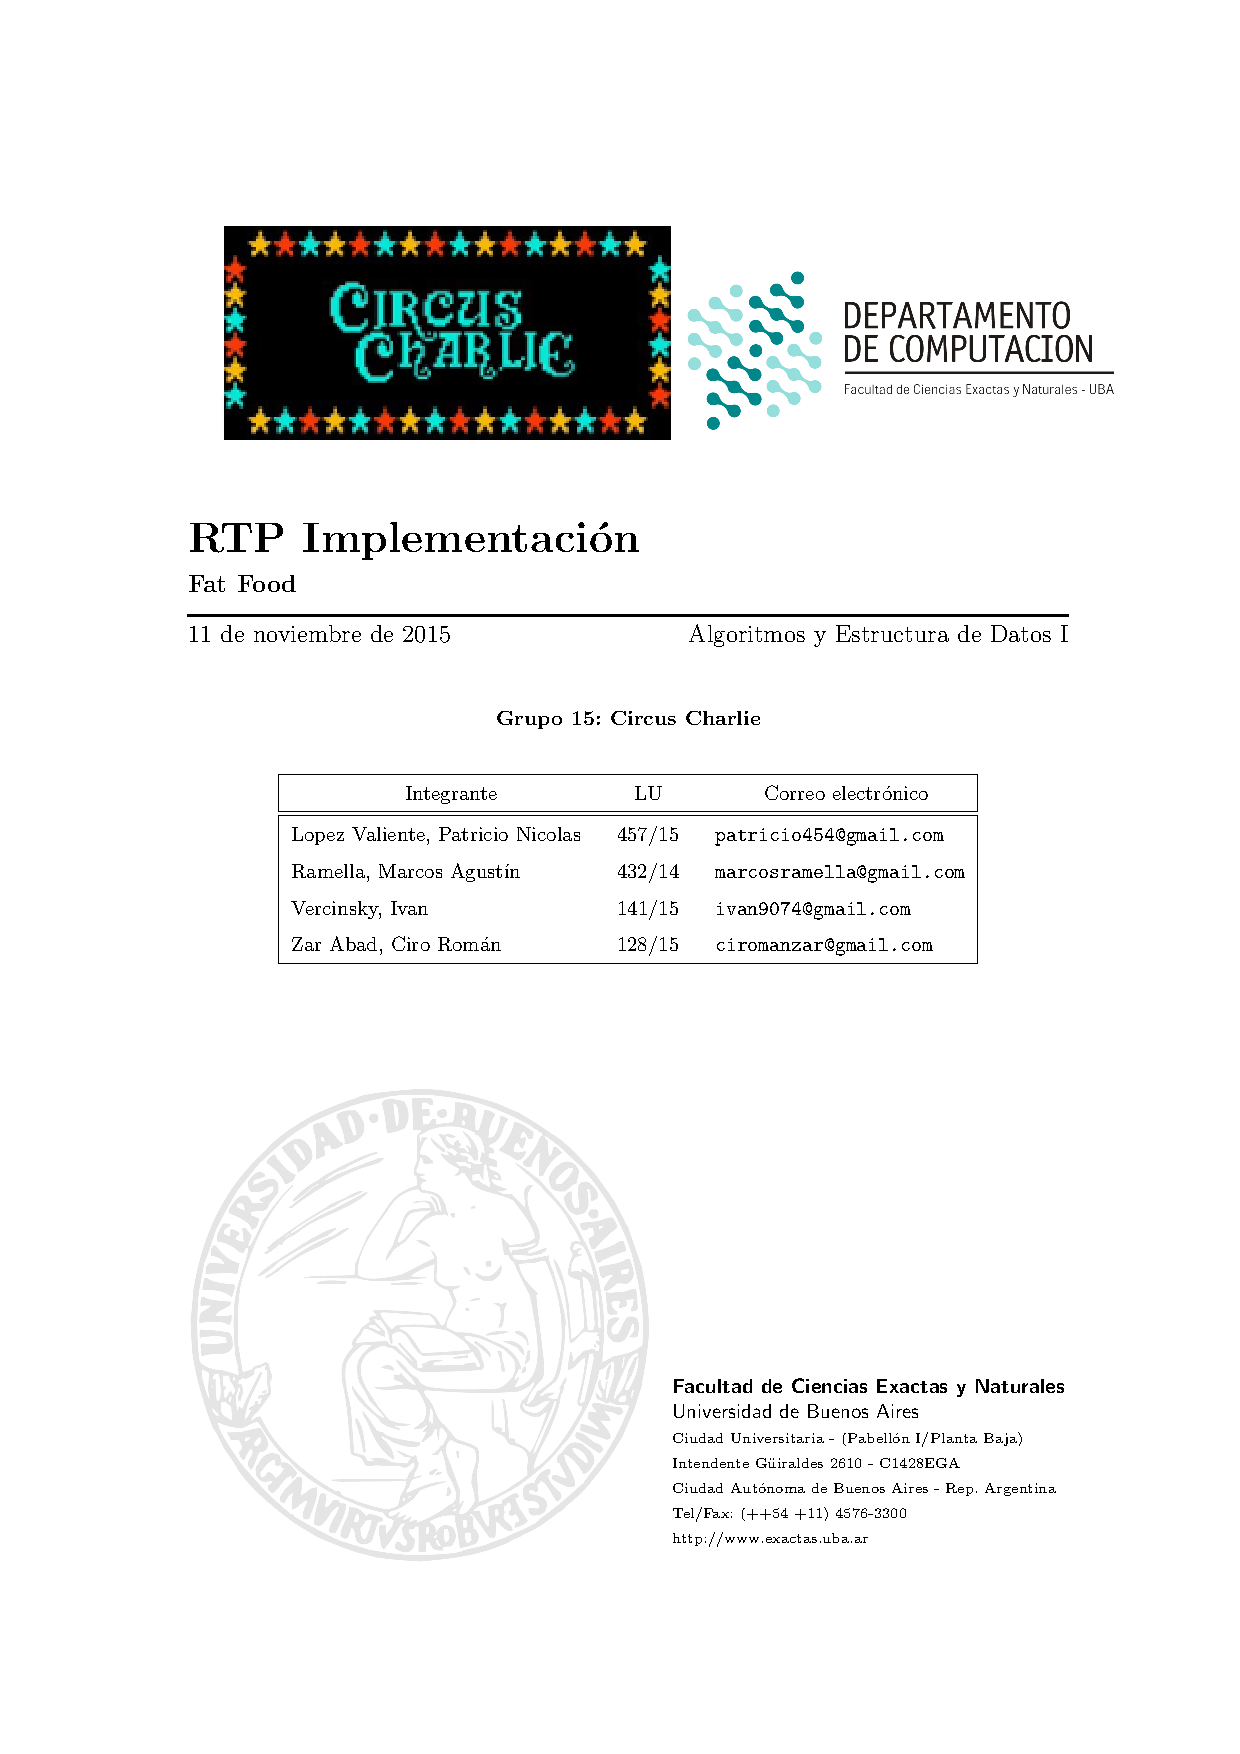
\includepdf{caratula}
\newpage %Salto de p�gina

\section{Implementaci�n}

\subsection{combo.cpp}
\begin{lstlisting}
#include "combo.h"
#include <string.h>
Combo::Combo(){
	_bebida = PestiCola ;
	_sandwich = McGyver ;
	_dificultad = 0;
}

Combo::Combo(const Bebida b, const Hamburguesa h, const Energia d ){
	_bebida = b ;
	_sandwich = h ;
	_dificultad = d;
}

Bebida Combo::bebidaC() const{
	Bebida res = this->_bebida ;
	return res ;
}

Hamburguesa Combo::sandwichC() const{
	Hamburguesa res = this->_sandwich ;
	return res ;
}

Energia     Combo::dificultadC() const{
	Energia res = this->_dificultad ;
	return res ;
}

void Combo::mostrar(std::ostream& os) const{
    os << "Bebida: " << _bebida << " | " << "Sandwich: " << _sandwich << " | " << "Dificultad: " << _dificultad ;
}


void Combo::guardar(std::ostream& os) const{
    os << " { C " << bebidaC() << " " <<  sandwichC() << " " << dificultadC() << " }" ;
}


void Combo::cargar (std::istream& is){
    //{ C FalsaNaranja CukiQueFresco 12 }
    string line;
    Bebida _b;
    string _sb;
    string _sh;    
    Hamburguesa _h;
    Energia _d;

    //leo el { 
    is >> line;
    //leo el 'C '
    is >> line;
    
    if (line == "C") {
        //sigo leyendo

        //leo la bebida
        is >> _sb;
        _b = recuperarBebidaDeString(_sb);
        //leo la hamburguesa
        is >> _sh;
        _h = recuperarHamburguesaDeString(_sh);
        //leo la dificultad
        is >> _d;

        //leo la }
        is >> line;

        this->_bebida = _b;
        this->_sandwich = _h;
        this->_dificultad = _d;
    } else {
        cout << "Archivo Invalido Combo";
    }
}

bool Combo::operator==(const Combo& otroCombo) const{
	bool igual = true ;
	if(this->_bebida != otroCombo._bebida){
		igual = false ;
	}
	else if(this->_sandwich != otroCombo._sandwich){
		igual = false ;
		}
	else if(this->_dificultad != otroCombo._dificultad){
		igual = false ;
		}
	return igual ;
}

std::ostream & operator<<(std::ostream & os,const Combo & c){
    c.mostrar(os);
	return os;
}

std::ostream & operator<<(std::ostream & os,const Hamburguesa & h){
    switch (h) {
        case McGyver:{
            os <<"McGyver";
            break;
        }
        case CukiQueFresco:{
            os <<"CukiQueFresco";
            break;            
        }
        case McPato:{
            os << "McPato";
            break;
        }
        case BigMacabra:{
            os <<"BigMacabra";
            break;            
        }
    }
    return os;

}

std::ostream & operator<<(std::ostream & os,const Bebida & b){
    switch (b) {
        case PestiCola:{
            os <<"PestiCola";
            break;
        }
        case FalsaNaranja:{
            os <<"FalsaNaranja";
            break;            
        }
        case SeVeNada:{
            os << "SeVeNada";
            break;
        }
        case AguaConGags:{
            os <<"AguaConGags";
            break;            
        }
        case AguaSinGags:{
            os <<"AguaSinGags";
            break;            
        }
    }
    return os;
}


Bebida recuperarBebidaDeString(string b) {
    Bebida _b;
    if (b ==  "PestiCola") { 
        _b = PestiCola;
    }
    if (b ==  "FalsaNaranja") { 
        _b = FalsaNaranja;
        
    }
    if (b ==  "SeVeNada") { 
        _b = SeVeNada;
        
    }
    if (b ==  "AguaConGags") { 
        _b = AguaConGags;
        
    }
    if (b ==  "AguaSinGags" ) { 
        _b = AguaSinGags;
        
    }
    return _b;
}

Hamburguesa recuperarHamburguesaDeString(string h) {
    Hamburguesa _h; 
    if(h=="McGyver") {
        _h = McGyver;
    }
    if(h=="CukiQueFresco") {
        _h = CukiQueFresco;
    }
    if(h=="McPato") {
        _h = McPato;
    }
    if(h=="BigMacabra") {
        _h = BigMacabra;
    }        
    return _h;
}
\end{lstlisting}
\newpage %Salto de p�gina

\subsection{combo.h}
\begin{lstlisting}
#ifndef COMBO_H_INCLUDED
#define COMBO_H_INCLUDED

#include "tipos.h"
#include <vector>

class Combo {

	public:

		Combo();
		Combo(const Bebida b, const Hamburguesa h, const Energia d);

		Bebida      bebidaC() const;
		Hamburguesa sandwichC() const;
		Energia     dificultadC() const;

		void        mostrar(std::ostream& os) const;
		void        guardar(std::ostream& os) const;
		void        cargar (std::istream& is);

		bool        operator==(const Combo& otroCombo) const;

	private:

		Bebida      _bebida;
		Hamburguesa _sandwich;
		Energia     _dificultad;

		enum {ENCABEZADO_ARCHIVO = 'C'};

};

// Definirlo usando mostrar, para poder usar << con este tipo.
std::ostream & operator<<(std::ostream & os,const Combo & c);
std::ostream & operator<<(std::ostream & os,const Hamburguesa & c);
std::ostream & operator<<(std::ostream & os,const Bebida & c);


#endif // COMBO_H_INCLUDED

\end{lstlisting}
\newpage %Salto de p�gina

\subsection{pedido.cpp}
\begin{lstlisting}
#include "pedido.h"
#include <algorithm>
Pedido::Pedido(){
	_combos = vector <Combo> ();
	_combos.push_back(Combo()) ;
	_atendio = "" ;
	_numero = 1 ;
}

Pedido::Pedido(const int nro, const Empleado e, const vector<Combo> combos){
	_combos = combos;
	_atendio = e ;
	_numero = nro ;
}

int Pedido::numeroP() const{
	int res = this->_numero ;
	return res ;
}

Empleado Pedido::atendioP() const{
	Empleado res = this->_atendio ;
	return res ;
}

vector<Combo> Pedido::combosP() const{
	vector<Combo> res = this->_combos ;
	return res ;
}

Energia Pedido::dificultadP() const{
	int i = 0 ;
	vector<Combo> p =  this->_combos ;
	int n = p.size() ;
	int suma = 0 ;
	while(i < n) {
		suma = suma + p.at(i).dificultadC() ;
		i++ ;
	}
	return suma ;
}


void  Pedido::agregarComboP(const Combo c){
	this->_combos.push_back(c) ;
}

void  Pedido::anularComboP(int i){
	int j = 0 ;
	vector<Combo> p =  this->_combos ;
	int n = p.size() ;
	vector<Combo> cs = vector <Combo> () ;
	while(j < n){
		if(j != i){
			cs.push_back(p.at(j)) ;
		}
		j++ ;
	}
	this->_combos = cs ;
}

void  Pedido::cambiarBebidaComboP(const Bebida b, int i){
	Hamburguesa ham = _combos.at(i).sandwichC() ;
	Energia dif = _combos.at(i).dificultadC() ;
	Combo ci = Combo( b , ham , dif ) ;
	_combos.at(i) = ci;
}

void  Pedido::elMezcladitoP(){
	vector< pair<Bebida, Hamburguesa> > noUsados = this->_posiblesParesNoUsados();
	int i = 0;
	int n = this->_combos.size();
	while(i < n){
		if(this->_estaRepetido(i)){
			int m = noUsados.size();
			Bebida b = noUsados.at(m - 1).first ;
			Hamburguesa h = noUsados.at(m - 1).second ;
			Energia d = this->_combos.at(i).dificultadC();
			this->_combos.at(i) = Combo(b, h, d) ;
			noUsados.pop_back() ;
		}
		i++ ;
	}

}


void Pedido::mostrar(std::ostream& os) const{
	os << "PEDIDO" << endl;
    os << "Numero: " << _numero << endl;
    os << "Empleado: " << _atendio << endl ;
    os << "Combos: " << endl ;
    os << endl ;
    for ( int i = 0 ; i < this->combosP().size() ; i++){
    	this->combosP().at(i).mostrar(os) ;
    	os << endl;
    }
}

void Pedido::guardar(std::ostream& os) const{
	os << "{ P " << numeroP() << " " <<  atendioP() << " [" ;
	for ( int i = 0 ; i < combosP().size() ; i++ ){
		combosP().at(i).guardar(os);
	}  
	os << " ] } " ;
}

void Pedido::cargar (std::istream& is){
    //{ P 1 pepe [ { C FalsaNaranja CukiQueFresco 10 } { C FalsaNaranja CukiQueFresco 12 } ] }
    
    string line;
    vector <Combo> _cs = vector <Combo> ();
    int _n;
    Empleado _e;

    //leo el {
    is >> line;
    //leo el 'P'
    is >> line;
    if (line == "P") {
        //sigo leyendo

        //leo el numero
        is >> _n;
        
        //leo el empleado
        is >> _e;

        //leo los combos

        //leo el [
        is >> line;
        
        while (true) {
            Combo _c = Combo();
            _c.cargar(is);
            _cs.push_back(_c);

            streampos pos = is.tellg();
            is >> line;
            if (line == "]") {
                break;
            } else {
                is.seekg(pos);
            }
        }
        //leo el } de pedido
        is >> line;

        this->_combos = _cs;
        this->_atendio = _e;
        this->_numero = _n;
    } 
    else {
        cout << "Archivo Invalido Pedido";
    }
}

bool Pedido::operator==(const Pedido& otroPedido) const{
	bool igual = true ;
	if(this->_atendio != otroPedido._atendio){
		igual = false ;
	}
	else if(this->_numero != otroPedido._numero){
		igual = false ;
		}
	else if( not this->_mismosCombos(otroPedido)){
		igual = false ;
		}
	return igual ;
}

std::ostream & operator<<(std::ostream & os,const Pedido& p){
	p.mostrar(os);
	return os ;
}

/**PARTE PRIVADA**/

vector< pair<Bebida, Hamburguesa> > Pedido::_posiblesParesNoUsados() {
	vector< pair<Bebida, Hamburguesa> > v = vector< pair<Bebida, Hamburguesa> >();
	vector<Bebida> bUsadas = this->_bebidasUsadas();
	vector<Hamburguesa> hUsadas = this->_sandwichesUsados();
	unsigned int i = 0;
	unsigned int j = 0;
	while(i < bUsadas.size()){
		j = 0 ;
		while(j < hUsadas.size()){
			pair<Bebida, Hamburguesa> par (bUsadas.at(i), hUsadas.at(j));
			v.push_back(par);
			j++;
		}
		i++;
	}
	vector< pair<Bebida, Hamburguesa> > v2 = this->_quitarUsados(v);
	return v2;
}

bool Pedido::_estaRepetido(unsigned int i) {
	bool res = false;
	unsigned int j = 0;
	vector<Combo> p = this->_combos;
	while(j < i){
		if(p.at(j).bebidaC() == p.at(i).bebidaC() && p.at(j).sandwichC() == p.at(i).sandwichC()){
			res = true;
		}
		j++;
	}
	return res;
}

vector<Bebida> Pedido::_bebidasUsadas() {
	vector<Bebida> b = vector<Bebida> () ;
	for(unsigned int i = 0 ; i < this->_combos.size() ; i++ ){
		bool tf = false;
		for(unsigned int j = 0 ; j < b.size() ; j++){
			if(b.at(j) == this->_combos.at(i).bebidaC()){
				tf = true;
			}
		}
		if(tf==false){
			b.push_back( this->_combos.at(i).bebidaC() ) ;
		}
	}
	return b;
}

vector<Hamburguesa> Pedido::_sandwichesUsados() {
	vector<Hamburguesa> h = vector<Hamburguesa> () ;
	for(unsigned int i = 0 ; i < this->_combos.size() ; i++ ){
		bool tf = false;
		for(unsigned int j = 0 ; j < h.size() ; j++){
			if(h.at(j) == this->_combos.at(i).sandwichC()){
				tf = true;
			}
		}
		if(tf==false){
			h.push_back( this->_combos.at(i).sandwichC() ) ;
		}
	}
	return h;
}
vector< pair<Bebida, Hamburguesa> > Pedido::_quitarUsados(vector< pair<Bebida, Hamburguesa> > v) {
	vector< pair<Bebida, Hamburguesa> > v2 = vector< pair<Bebida, Hamburguesa> >();
	vector<Combo> c = this->_combos ;
	int i = 0;
	int j = 0;
	int n = v.size();
	int m = c.size() ;
	while(i < n){
		bool tf = false;
		j = 0 ;
		while(j < m){
			if(v.at(i).first == c.at(j).bebidaC() && v.at(i).second == c.at(j).sandwichC() ){
				tf = true;
			}
			j++;
		}
		if(tf == false){
			v2.push_back(v.at(i));
		}
		i++;
	}
	return v2;
}


bool Pedido::_mismosCombos(const Pedido& otroPedido) const{
	bool res = true;
	if(this->_combos.size() != otroPedido._combos.size()){
		res = false;
	}
	for(unsigned int i = 0 ; i < this->_combos.size() ; i++ ){
		if(this->_cuenta(this->_combos.at(i)) != otroPedido._cuenta(this->_combos.at(i))){
			res = false;
		}
	}
	return res;
}

int Pedido::_cuenta(Combo c)const{
	int cuenta = 0;
	for(unsigned int i = 0; i < this->_combos.size() ; i++){
		if(this->_combos.at(i) == c){
			cuenta++;
		}
	}
	return cuenta;
}

\end{lstlisting}
\newpage %Salto de p�gina

\subsection{pedido.h}
\begin{lstlisting}
#ifndef PEDIDO_H_INCLUDED
#define PEDIDO_H_INCLUDED

#include <vector>
#include "tipos.h"
#include "combo.h"

class Pedido {

	public:

		Pedido();
		Pedido(const int n, const Empleado e, const vector<Combo> cs);
 
		int                 numeroP() const;
		Empleado            atendioP() const;
		vector<Combo>       combosP() const;
		Energia             dificultadP() const;

		void                agregarComboP(const Combo c);
		void                anularComboP(int i);
		void                cambiarBebidaComboP(const Bebida b, int i);
		void                elMezcladitoP();

		void                mostrar(std::ostream& os) const;
		void                guardar(std::ostream& os) const;
		void                cargar (std::istream& is);

		bool                operator==(const Pedido& otroPedido) const;

	private:

                vector<Combo>       _combos;
                Empleado            _atendio;
                int                 _numero;


                vector< pair<Bebida, Hamburguesa> >     _posiblesParesNoUsados() ;
                bool                                    _estaRepetido(unsigned int);
                vector<Bebida>                          _bebidasUsadas();
                vector<Hamburguesa>                     _sandwichesUsados();
                vector< pair<Bebida, Hamburguesa> >     _quitarUsados(vector< pair<Bebida, Hamburguesa> >);
                bool                                    _mismosCombos(const Pedido& otroPedido) const;
                int                                     _cuenta(Combo) const;

                enum {ENCABEZADO_ARCHIVO = 'P'};
};

// Definirlo usando mostrar, para poder usar << con este tipo.
std::ostream & operator<<(std::ostream & os,const Pedido & p);

#endif // PEDIDO_H_INCLUDED

\end{lstlisting}
\newpage %Salto de p�gina

\subsection{local.cpp}
\begin{lstlisting}
#include "local.h"
#include <string.h>
Local::Local(){
	_bebidas = vector <pair <Bebida,Cantidad> > ();
	_sandwiches = vector <pair <Hamburguesa,Cantidad> > ();
	_empleados = vector< pair <Empleado, Energia> >();
	_ventas = vector< Pedido > ();

	pair <Bebida, Cantidad> b1 (PestiCola, 2);
	pair <Bebida, Cantidad> b2 (FalsaNaranja, 2);
	pair <Bebida, Cantidad> b3 (SeVeNada, 2);
	pair <Bebida, Cantidad> b4 (AguaConGags, 2);
	pair <Bebida, Cantidad> b5 (AguaSinGags, 2);
	_bebidas.push_back(b1);
	_bebidas.push_back(b2);
	_bebidas.push_back(b3);
	_bebidas.push_back(b4);
	_bebidas.push_back(b5);

	pair <Hamburguesa, Cantidad> h1 (McGyver, 2);
	pair <Hamburguesa, Cantidad> h2 (CukiQueFresco, 2);
	pair <Hamburguesa, Cantidad> h3 (McPato, 2);
	pair <Hamburguesa, Cantidad> h4 (BigMacabra, 2);
	_sandwiches.push_back(h1);
	_sandwiches.push_back(h2);
	_sandwiches.push_back(h3);
	_sandwiches.push_back(h4);

	pair <Empleado, Energia> e1 ("Ronald Maconal", 100);
	pair <Empleado, Energia> e2 ("Burguer Kong", 100);
	_empleados.push_back(e1);
	_empleados.push_back(e2);

}

Local::Local(const vector< pair <Bebida,Cantidad> > bs, const vector< pair <Hamburguesa,Cantidad> > hs, const vector<Empleado> es){
	_bebidas = bs;
	_sandwiches = hs;
	unsigned int i = 0;
	_empleados = vector< pair <Empleado, Energia> >();
	while (i < es.size()) {
		pair <Empleado, Energia> e (es.at(i), 100);
		_empleados.push_back(e);
		i++;
	}
	_ventas = vector< Pedido > ();
}

Cantidad Local::stockBebidasL(const Bebida b) const{
	unsigned int i = 0;
	while (i < _bebidas.size() && _bebidas.at(i).first != b) {
		i++;
	}
	return _bebidas.at(i).second;
}

Cantidad Local::stockSandwichesL(const Hamburguesa h) const{
	unsigned int i = 0;
	while (i < _sandwiches.size() && _sandwiches.at(i).first != h) {
		i++;
	}
	return _sandwiches.at(i).second;
}

vector<Bebida> Local::bebidasDelLocalL() const{
	unsigned int i = 0;
	vector<Bebida> b = vector<Bebida>();
	while(i < _bebidas.size()){
		b.push_back(_bebidas.at(i).first);
		i++;
	}
	return b;
}

vector<Hamburguesa> Local::sandwichesDelLocalL() const{
	unsigned int i = 0;
	vector<Hamburguesa> s = vector<Hamburguesa>();
	while(i < _sandwiches.size()){
		s.push_back(_sandwiches.at(i).first);
		i++;
	}
	return s;
}


vector<Empleado> Local::empleadosL() const{
	int i = 0;
	vector<Empleado> emp = vector<Empleado>();
	while (i < _empleados.size()) {
		if(_empleados.at(i).second >= 0 ) {
			emp.push_back(_empleados.at(i).first);	
		}
		i++;
	}
	return emp;
}

vector<Empleado> Local::desempleadosL() const{
	int i = 0;
	vector<Empleado> demp = vector<Empleado>();
	
	while(i < _empleados.size()){
		if ( _empleados.at(i).second < 0) {
			demp.push_back(_empleados.at(i).first);	
		}
		i++;
	}

	return demp;
}

Energia  Local::energiaEmpleadoL(const Empleado e) const{
	int i = 0;
	while(e != _empleados.at(i).first) {
		i++;
	}
	return _empleados.at(i).second;
}

vector<Pedido> Local::ventasL() const{
	return _ventas;
}

vector<Empleado> Local::candidatosAEmpleadosDelMesL() const{
        return _candidatosAEmpleadosDelMes();
}

void Local::venderL(const Pedido p){

	//Buscar Empleado que Atentio el Pedido p
	int i = 0;
	while( i < _empleados.size() && p.atendioP() != _empleados.at(i).first ){
			i++ ;
	}
	//Resta Energia
	_empleados.at(i).second -= p.dificultadP() ;
	
	if( _empleados.at(i).second >= 0 ){
	//**Empleado con Energia para atender
		//**Actualiza ventas
		_ventas.push_back(p) ;
		//**Actualiza Bebidas y Sandwiches
		i = 0 ;		
		while( i < p.combosP().size() ){
			_actualizaStockBebida( p.combosP().at(i).bebidaC() , -1 ) ;
			_actualizaStockSandwich( p.combosP().at(i).sandwichC() , -1 ) ;
			i++ ;
		}
	}		
}	

void Local::sancionL(const Empleado e, const Energia n){
	int i = 0 ;
	while( i < _empleados.size() && e != _empleados.at(i).first ){
		i++ ;
	}
	_empleados.at(i).second -= n;
	
}

void Local::anularPedidoL(int n){
	vector <Pedido> vMinN = vector <Pedido> () ;
	int i = 0 ;
	vector <Combo> combos ;
	int nro ; 
	Empleado emp ;
	while ( i < _ventas.size() ){
		if ( _ventas.at(i).numeroP() < n ){
			vMinN.push_back(_ventas.at(i)) ;
		}	
		else if ( _ventas.at(i).numeroP() == n ){
			int j = 0 ;
			while( j < _empleados.size() && _ventas.at(i).atendioP() != _empleados.at(j).first ){
				j++ ;
			}
			_empleados.at(j).second += _ventas.at(i).dificultadP() ;
			j = 0 ;
			while( j < _ventas.at(i).combosP().size() ){
				_actualizaStockBebida( _ventas.at(i).combosP().at(j).bebidaC() , 1 ) ;
				_actualizaStockSandwich( _ventas.at(i).combosP().at(j).sandwichC() , 1 ) ;
				j++ ;
			}
		}	
		else {
			emp = _ventas.at(i).atendioP() ;
			combos = _ventas.at(i).combosP() ;
			nro = _ventas.at(i).numeroP() - 1 ;
			vMinN.push_back( Pedido( nro , emp , combos ) ) ;
		}
	i++ ;
	}
	_ventas = vMinN ;
}

void Local::agregarComboAlPedidoL(const Combo c, int n){
	int i = 0 ;
	_actualizaStockBebida( c.bebidaC() , -1 ) ;
	_actualizaStockSandwich( c.sandwichC() , -1 ) ;
	while( i < _ventas.size() && _ventas.at(i).numeroP() != n ){
		i++ ;
	}
	_ventas.at(i).agregarComboP(c) ;
	int j = 0 ;
	while( j < _empleados.size() && _ventas.at(i).atendioP() != _empleados.at(j).first ){
		j++ ;
	}
	_empleados.at(j).second -= c.dificultadC() ;
}

bool Local::unaVentaCadaUnoL() const{
	int i = 0 ;
	bool ciclan = true ;
	while( i < _pedidosOrdenadosDeEmpleadosActuales().size() ){
		int imod = i % _empleadosDelCiclo().size() ;
		if ( _pedidosOrdenadosDeEmpleadosActuales().at(i).atendioP() != _pedidosOrdenadosDeEmpleadosActuales().at(imod).atendioP() ){
			ciclan = false ;
		}
	i++ ;
	}
	return ciclan ;
}

Empleado Local::elVagonetaL() const{
	int i = 0;
	vector<Empleado> emps = empleadosL();
	Empleado vagoneta;
	int max = 0;

	while(i < emps.size()) {
		int desc = _descansoMasLargo(emps.at(i));
		if (desc >= max) {
			max = desc;
			vagoneta = emps.at(i);
		}
		i++;
	}	
	return vagoneta;
}
	
void Local::guardar(std::ostream& os) const{
	os << "{ ";
	os << "L ";
	os << "[ ";
	int i = 0;
	while(i < bebidasDelLocalL().size()) {
		os << "( ";
		os << bebidasDelLocalL().at(i) << " ";
		os << stockBebidasL(bebidasDelLocalL().at(i)) << " ";
		os << ") ";
		i++;
	}
	os << "] ";
	os << "[ ";
	i = 0;
	while(i < sandwichesDelLocalL().size()) {
		os << "( ";
		os << sandwichesDelLocalL().at(i) << " ";
		os << stockSandwichesL(sandwichesDelLocalL().at(i)) << " ";
		os << ") ";
		i++;
	}
	os << "] ";
	os << "[ ";
	i = 0;
	while(i < _empleados.size()) {
		os << "( ";
		os << _empleados.at(i).first << " ";
		os << energiaEmpleadoL(_empleados.at(i).first) << " ";
		os << ") ";
		i++;
	}
	os << "] ";
	os << "[ ";
	i = 0;
	while(i < ventasL().size()) {
		ventasL().at(i).guardar(os);
		i++;
	}
	os << "] ";
	os << "}" << endl;
}	

void Local::mostrar(std::ostream& os) const{
	os << "Local" << endl;
	os << endl;
     os << "Bebidas : " << endl;
    	for (int i = 0; i < bebidasDelLocalL().size(); i++)
    	{
			os << bebidasDelLocalL().at(i) << " | Cantidad: " << stockBebidasL(bebidasDelLocalL().at(i)) << endl;
    	}
    	os << endl;
    	os << "Hamburguesas : " << endl;
    	for (int i = 0; i < sandwichesDelLocalL().size(); i++)
    	{
			os << sandwichesDelLocalL().at(i) << " | Cantidad: " << stockSandwichesL(sandwichesDelLocalL().at(i)) << endl;
    	}
    	os << endl;
    	os << "Empleados : " << endl;
    	for (int i = 0; i < empleadosL().size(); i++)
    	{
			os << empleadosL().at(i) << " | Energia: " << energiaEmpleadoL(empleadosL().at(i)) << endl;
    	}
    	os << endl;
    	os << "Desempleados : " << endl;
    	for (int i = 0; i < desempleadosL().size(); i++)
    	{
			os << desempleadosL().at(i) << endl;
    	}
	os << endl;
    	os << "Cantidatos a Empleados del Mes : " << endl;
    	for (int i = 0; i < candidatosAEmpleadosDelMesL().size(); i++)
    	{
		os << candidatosAEmpleadosDelMesL().at(i) << endl;
    	}
    	os << endl;
    	os << "El Vagoneta : " << elVagonetaL() << endl;

	os << endl;
    	os << "Ventas : " << endl;
    	os << endl;
    	for (int i = 0; i < ventasL().size(); i++)
    	{
		ventasL().at(i).mostrar(os);
    	os << endl;		
    	}

}

void Local::cargar (std::istream& is){

	string line;
	vector <pair <Bebida,Cantidad> > _bs = vector <pair <Bebida,Cantidad> > ();
	vector <pair <Hamburguesa,Cantidad> > _hs = vector <pair <Hamburguesa,Cantidad> > ();
	vector< pair <Empleado, Energia> > _es = vector< pair <Empleado, Energia> > ();
	vector< pair <Empleado, Energia> > _ds = vector< pair <Empleado, Energia> > ();
	vector< Pedido > _vs = vector< Pedido > ();

	//leo {
	is >> line;

	//leo L
	is >> line;

	//cargo stock y empleados;
	//[ ( AguaConGags 7 ) ] [ ( CukiQueFresco 7 ) ] [ ( pepe 56 ) ( juan 88 ) ]

	//cargo stock y empleados;
	//[ ( AguaConGags 7 ) ( AguaConGags 7 ) ] [ ( CukiQueFresco 7 ) ] [ ( pepe 56 ) ( juan 88 ) ]
	
	//leo [
	is >> line;

	while(true) {
		
		//leo (
		is >> line;
		
		//leo AguaConGags
		is >> line;
		Bebida b = recuperarBebidaDeString(line);

		Cantidad c;
		is >> c;	

		pair <Bebida, Cantidad> bc = pair<Bebida, Cantidad> (b, c);
		_bs.push_back(bc);
		//leo )
		is >> line;	

		streampos pos = is.tellg();
        is >> line;
        if (line == "]") {
            break;
        } else {
            is.seekg(pos);
        }
	}


	//leo [
	is >> line;

	

	while(true) {
		//leo (
		is >> line;
		
		//leo Hamburguesa
		is >> line;
		Hamburguesa h = recuperarHamburguesaDeString(line);

		Cantidad c;
		is >> c;	

		pair <Hamburguesa, Cantidad> hc = pair<Hamburguesa, Cantidad> (h, c);
		_hs.push_back(hc);
		//leo )
		is >> line;	

		streampos pos = is.tellg();
        is >> line;
        if (line == "]") {
            break;
        } else {
            is.seekg(pos);
        }
	}

	
	//[ ( pepe 56 ) ( juan 88 ) ]
	//leo [
	is >> line;

	while(true) {
		//leo (
		is >> line;

		is >> line;
		Empleado e = line;

		Energia c;
		is >> c;	

		pair <Empleado, Energia> ee = pair<Empleado, Energia> (e, c);
		_es.push_back(ee);
		//leo )
		is >> line;	

		streampos pos = is.tellg();
        is >> line;
        if (line == "]") {
            break;
        } else {
            is.seekg(pos);
        }
	}


	//leer las ventas;
	//leo [
	is >> line;

	//me fijo si hay pedidos. Si fuera [ ] Entonces no entro al While
	streampos pos = is.tellg();
    is >> line;
    
	if (line != "]") {
        is.seekg(pos);
		while(true) {

			Pedido _p = Pedido();
	        _p.cargar(is);
			_vs.push_back(_p);

			streampos pos = is.tellg();
	        is >> line;
	        if (line == "]") {
	            break;
	        } else {
	            is.seekg(pos);
	        }
		}
	}


	this->_bebidas = _bs;
	this->_sandwiches = _hs;
	this->_empleados = _es;
	this->_ventas = _vs;

}

std::ostream & operator<<(std::ostream & os,const Local & l){
	l.mostrar(os);
	return os;
}



/**Parte Privada**/


vector <Empleado> Local::_candidatosAEmpleadosDelMes() const{
	return _empleadosConMasCombos(_empleadosConMasVentas(empleadosL()));
}

vector < Empleado > Local::_empleadosConMasCombos(const vector <Empleado> empleados) const{
	int i = 0;
	vector < Empleado > emp = vector < Empleado >();

	//**Busco el maximo de Combos vendidos por todos los empleados.
	int maxCombos = 0;
	while (i < empleados.size()) {



		if ( _combosVendidosPorElEmpleado(empleados.at(i)).size() > maxCombos) {
			maxCombos = _combosVendidosPorElEmpleado(empleados.at(i)).size(); 			
		}
		i++;
	}

	//**Me quedo con los empleados que hayan vendido al menos maxCombo de combos
	i=0;
	while (i < empleados.size()) {
		if ( _combosVendidosPorElEmpleado(empleados.at(i)).size() >= maxCombos) {
			emp.push_back(empleados.at(i));
		}
		i++;
	}
	return emp;

}
vector < Empleado > Local::_empleadosConMasVentas(const vector <Empleado> empleados) const{
	int i = 0;
	vector < Empleado > emp = vector < Empleado >();

	//**Busco el maximo de Combos vendidos por todos los empleados.
	int maxVentas = 0;
	while (i < empleados.size()) {
		if ( _ventasDelEmpleado(empleados.at(i)).size() > maxVentas) {
			maxVentas = _ventasDelEmpleado(empleados.at(i)).size();
		}
		i++;
	}


	//**Me quedo con los empleados que hayan vendido al menos maxCombo de combos
	i=0;
	while (i < empleados.size()) {
		if ( _ventasDelEmpleado(empleados.at(i)).size() >= maxVentas) {
			emp.push_back(empleados.at(i));
		}
		i++;
	}
	return emp;

}

vector < Pedido > Local::_ventasDelEmpleado(const Empleado e) const{
	vector <Pedido> ventas = vector <Pedido>();
	int i = 0;
	while(i < ventasL().size()) {
		if (ventasL().at(i).atendioP() == e) {
			ventas.push_back(ventasL().at(i));
		}
		i++;
	}
	return ventas;

}
vector < Combo >  Local::_combosVendidosPorElEmpleado(const Empleado e) const{
	vector <Combo> combos = vector <Combo>();
	int i = 0;
	while(i < ventasL().size()) {
		if (ventasL().at(i).atendioP() == e) {
			int j = 0;
			while (j < ventasL().at(i).combosP().size()) {
				combos.push_back(ventasL().at(i).combosP().at(j));
				j++;
			}
		}
		i++;
	}
	return combos;
}

Pedido Local::_pedidoPorNro(const int n) const {
	vector <Pedido> ventas = vector <Pedido>();
	int i = 0;
	while(i < ventasL().size() && ventasL().at(i).numeroP() != n) {
		i++;
	}
	return ventasL().at(i);
}

int Local::_minNroPedido(const vector <Pedido> ps) const {
	int min = 0;
	int i = 0;
	if (ps.size() == 0) {
		return 0;
	} else {
		min = ps.at(i).numeroP();
	}
	while( i < ps.size()) {
		if (ps.at(i).numeroP() < min) {
			min = ps.at(i).numeroP();
		}
		i++;
	}
	return min;
}
int Local::_maxNroPedido(const vector <Pedido> ps) const {
	int max = 0;
	int i = 0;
	while( i < ps.size()) {
		if (ps.at(i).numeroP() > max) {
			max = ps.at(i).numeroP();
		}
		i++;
	}
	return max;
}

vector < Pedido > Local::_pedidosOrdenados() const{
	//declaro
	int min = 0;
	int max = 0;
	int i = 0;
	vector <Pedido> pedidos = vector < Pedido >();
	//inicializo
	min = _minNroPedido(ventasL());
	max = _maxNroPedido(ventasL());
	i = min;

	while(i <= max) {
		pedidos.push_back(_pedidoPorNro(i));
		//uso invariante...el numero de las ventas son consecutivos!!!!
		i++;
	}

	return pedidos;


}
vector < Pedido > Local::_pedidosOrdenadosDeEmpleado(const Empleado e) const {
	int i = 0;
	vector <Pedido> pedidos = vector < Pedido >();
	vector <Pedido> pedidosOrdenados = _pedidosOrdenados();

	while (i < pedidosOrdenados.size()) {
		if (pedidosOrdenados.at(i).atendioP() == e) {
			pedidos.push_back(pedidosOrdenados.at(i));
		}
		i++;
	}
	return pedidos;
}
int Local::_descansoMasLargo(const Empleado e) const {
	int i = 0;
	int max = 0;
	vector < int > descansos = _descansos(e);
	while(i < descansos.size()) { 
		if ( descansos.at(i) > max) {
			max = descansos.at(i);
		}
		i++;
	}
	return max;
}
vector < int > Local::_descansos(const Empleado e) const {
	vector <int> descansos = vector<int>();
	if (_ventasDelEmpleado(e).size() == 0) {
		descansos.push_back(ventasL().size());
	} else {
		//primer descanso
		vector <Pedido> pedidosOrdenadosEmp = _pedidosOrdenadosDeEmpleado(e);
		int min = _minNroPedido(ventasL());
		descansos.push_back(pedidosOrdenadosEmp.at(0).numeroP() - min);

		//descansos intermedios.
		int  i = 0;
		while (i < pedidosOrdenadosEmp.size() - 1) {
			descansos.push_back(pedidosOrdenadosEmp.at(i+1).numeroP() - pedidosOrdenadosEmp.at(i).numeroP());
			i++;
		}

		//ultimo descanso
		int max = _maxNroPedido(ventasL());
		descansos.push_back(max - pedidosOrdenadosEmp.at(pedidosOrdenadosEmp.size()-1).numeroP());
	}
	return descansos;
}

void Local::_actualizaStockBebida(const Bebida b , const int n ) {
	unsigned int i = 0;
	while (i < _bebidas.size() && _bebidas.at(i).first != b) {
		i++;
	}
	_bebidas.at(i).second += n ;

}	
void Local::_actualizaStockSandwich(const Hamburguesa h , const int n ) {
	unsigned int i = 0;
	while (i < _sandwiches.size() && _sandwiches.at(i).first != h) {
		i++;
	}
	_sandwiches.at(i).second += n ;
}	

vector<Pedido> Local::_pedidosOrdenadosDeEmpleadosActuales() const{
	//declaro
	int min = 0;
	int max = 0;
	int i = 0;
	vector <Pedido> pedidos = vector < Pedido >();
	//inicializo
	min = _minNroPedido(ventasL());
	max = _maxNroPedido(ventasL());
	i = min;

	while(i <= max) {
		bool in = false ;
		for(int j = 0 ; j < empleadosL().size() ; j++){
			if( _pedidoPorNro(i).atendioP() == empleadosL().at(j) ){
				in = true ;
			}
		}
		if(in == true){
			pedidos.push_back(_pedidoPorNro(i)) ;
		//Numero ventas es consecutivo
		}
		i++;
	}

	return pedidos;
}	

vector<Empleado> Local::_empleadosDelCiclo() const{
	unsigned int i = 0;
	vector < Empleado > emp = vector < Empleado >() ;
	while( i < _pedidosOrdenadosDeEmpleadosActuales().size() ){
		bool yaEsta = false ;
		for(int j = 0 ; j < emp.size() ; j++){
			if( _pedidosOrdenadosDeEmpleadosActuales().at(i).atendioP() == emp.at(j) ){
				yaEsta = true ;
			}
		}
		if( yaEsta == false ){
			emp.push_back(_pedidosOrdenadosDeEmpleadosActuales().at(i).atendioP()) ;
		}
		i++ ;
	}
	return emp ;
}

\end{lstlisting}
\newpage %Salto de p�gina

\subsection{local.h}
\begin{lstlisting}
#ifndef LOCAL_H_INCLUDED
#define LOCAL_H_INCLUDED

#include <vector>
#include "pedido.h"

class Local{
    
    public:

        Local();
        Local(const vector< pair <Bebida,Cantidad> > bs, const vector< pair <Hamburguesa,Cantidad> > hs, const vector<Empleado> es);

        Cantidad                stockBebidasL(const Bebida b) const;
        Cantidad                stockSandwichesL(const Hamburguesa h) const;
        vector<Bebida>          bebidasDelLocalL() const;
        vector<Hamburguesa>     sandwichesDelLocalL() const;
        vector<Empleado>        empleadosL() const;
        vector<Empleado>        desempleadosL() const;
        Energia                 energiaEmpleadoL(const Empleado e) const;
        vector<Pedido>          ventasL() const;
        bool                    unaVentaCadaUnoL() const;
        void                    venderL(const Pedido p);
        vector<Empleado>        candidatosAEmpleadosDelMesL() const;
        void                    sancionL(const Empleado e, const Energia n);
        Empleado                elVagonetaL() const;
        void                    anularPedidoL(int n);
        void                    agregarComboAlPedidoL(const Combo c, int n);
        void                    mostrar(std::ostream& os) const;
        void                    guardar(std::ostream& os) const;
        void                    cargar (std::istream& is);

    private:

        enum {ENCABEZADO_ARCHIVO = 'L'};
        vector< pair <Hamburguesa,Cantidad> >   _sandwiches;
        vector< pair <Bebida,Cantidad> >        _bebidas;
        vector< pair <Empleado, Energia> >      _empleados;
        vector< Pedido >                        _ventas;
        vector < Empleado >                     _candidatosAEmpleadosDelMes() const;
        vector < Empleado >                     _empleadosConMasCombos(const vector <Empleado> empleados) const;
        vector < Empleado >                     _empleadosConMasVentas(const vector <Empleado> empleados) const;
        vector < Pedido >                       _ventasDelEmpleado(const Empleado e) const;
        vector < Combo >                        _combosVendidosPorElEmpleado(const Empleado e) const;
        int                                     _minNroPedido(const vector <Pedido> ps) const;
        int                                     _maxNroPedido(const vector <Pedido> ps) const;
        Pedido                                  _pedidoPorNro(const int n) const;
        vector < Pedido >                       _pedidosOrdenados() const;
        vector < Pedido >                       _pedidosOrdenadosDeEmpleado(const Empleado e) const;
        int                                     _descansoMasLargo(const Empleado e) const;
        vector < int >                          _descansos(const Empleado e) const;
        vector<Pedido>                          _pedidosOrdenadosDeEmpleadosActuales() const;
        vector<Empleado>                        _empleadosDelCiclo() const;
        void                                    _actualizaStockBebida(const Bebida b , const int n );
        void                                    _actualizaStockSandwich(const Hamburguesa h , const int n );
};
#endif // LOCAL_H_INCLUDED
std::ostream & operator<<(std::ostream & os,const Local & c);

\end{lstlisting}
\newpage %Salto de p�gina


\section{Demostraciones} %Demostraciones

\subsection{candidatosAEmpleadosDelMesL}
\subsubsection{Primer ciclo}
\begin{lstlisting}
vector<Empleado> Local::candidatosAEmpleadosDelMesL() const{
        return _candidatosAEmpleadosDelMes();
}

vector <Empleado> Local::_candidatosAEmpleadosDelMes() const{
	return _empleadosConMasCombos(_empleadosConMasVentas(empleadosL()));
}

vector < Empleado > Local::_empleadosConMasCombos(const vector <Empleado> empleados) const{
	int i = 0;
	vector < Empleado > emp = vector < Empleado >();

	//**Busco el maximo de Combos vendidos por todos los empleados.
	int maxCombos = 0;
	while (i < empleados.size()) {
		if ( _combosVendidosPorElEmpleado(empleados.at(i)).size() > maxCombos) {
			maxCombos = _combosVendidosPorElEmpleado(empleados.at(i)).size();
		}
		i++;
	}
\end{lstlisting} 


\hspace{15pt}\textbf{Pc, Qc, I, B, cota y fv.} \\
Llamo $sizeE = |empleados(l)| $; \\
Vale $sizeE > 0$ por invariante de Local. ;\\
Implica  $|empleados(l)| > 0$ ;\\
Llamo $sizeCombosVendidosE(i) = | combosVendidosPorElEmpleado(l, empleados(l)_i) | $; \\
Llamo $combosVendidosPorElEmpleado = concat[combos(p)|p \leftarrow ventas(l), atendio(p) == e]$ ;\\

Pc: $i == 0 \wedge maxCombos == 0 \wedge emp == [] \wedge sizeE > 0$ ;\\
Qc: $(\forall j \leftarrow [0..sizeE)) |combosVendidosPorElEmpleado(l, empleados(l)[j])| \leq maxCombos$ ;\\
B: $i < sizeE$ ;\\
I: $0 \leq i \leq sizeE \wedge (\forall j \leftarrow [0..i)) |combosVendidosPorElEmpleado(l, empleados(l)[j])| \leq maxCombos$ ;\\ 	
fv: $sizeE - i$ ;\\
cota: 0 ;\\

\hspace{15pt}\textbf{Pc $\wedge$ B $\Rightarrow$ I:} \\
Por Pc $\wedge$ B : $i == 0 \wedge maxCombos == 0 \wedge emp == [] \wedge sizeE > 0 \wedge i < sizeE $ ;\\
Implica $ i == 0 \wedge i < sizeE \wedge sizeE > 0 \Leftrightarrow 0 == i < sizeE $ ; \\
Implica $ 0 \leq i \leq sizeE $ ;\\

Luego usando que $i == 0$ y por Pc sabemos que $maxCombos == 0$ ;\\
Y $(\forall j \leftarrow [0..0)) |combosVendidosPorElEmpleado(l, empleados(l)_j)| == 0 $ ;\\
Implica que $(\forall j \leftarrow [0..i)) |combosVendidosPorElEmpleado(l, empleados(l)_j)| == maxCombos $ ;\\
Implica que $(\forall j \leftarrow [0..i)) |combosVendidosPorElEmpleado(l, empleados(l)_j)| \leq maxCombos $ ;\\

Luego sabemos que $0 \leq i \leq sizeE \wedge (\forall j \leftarrow [0..i)) |combosVendidosPorElEmpleado(l, empleados(l)_j)| \leq maxCombos$ ;\\
Equivale a I ;\\

\hspace{15pt}\textbf{I $\wedge \neg $ B $\Rightarrow$ Qc:} \\
Usando que $i \leq sizeE$ por el Invariante y $i >= sizeE$ por la negacion de la guarda ;\\
Entonces $i \leq sizeE \wedge  i \geq sizeE \Rightarrow i == sizeE $ ;\\
Reemplazo en I: $(\forall j \leftarrow [0..sizeE)) |combosVendidosPorElEmpleado(l, empleados(l)_j)| \leq maxCombos $ ;\\
Lo cual es equivalente a Qc. ;\\

\hspace{15pt}\textbf{I $\wedge$ fv $\leq$ Cota $\Rightarrow \neg$ B:} \\
I $\wedge$ fv $\leq$: $0 \leq i \leq sizeE \wedge sizeE - i \leq cota$ ;\\
Implica $ 0 \leq i \leq sizeE \wedge sizeE \leq i.$ ;\\
Implica $i == sizeE.$ ;\\
Implica $i \geq sizeE.$ Lo cual es equivalente a $ \neg$ B. ;\\
\\
\\



\newpage %Salto de p�gina

\subsection{elVagonetaL}
\begin{lstlisting}
Empleado Local::elVagonetaL() const{
	int i = 0;
	vector<Empleado> emps = empleadosL();
	Empleado vagoneta;
	int max = 0;
	while(i < emps.size()) {
		int desc = _descansoMasLargo(emps.at(i));
		if (desc >= max) {
			max = desc;
			vagoneta = emps.at(i);
		}
		i++;
	}	
	return vagoneta;
}
\end{lstlisting}

\hspace{15pt}\textbf{Pc, Qc, I, B, cota y fv.} \\
Pc: $i==0 \wedge \ max==0 \wedge |emps| >  0 $ \  (por requiere) \ $ \wedge (\forall i, j, \leftarrow[0..|emps|), i \neq j) emps_i \neq emps_j$  (por invariante empleadosDistintos) ; \\
Qc: $(\forall \ e \leftarrow[0..|emps|)) descansoMasLargo(l, emps[e]) \leq descansoMasLargo(l, vagoneta) \wedge \\ descansoMasLargo(l, emps[e]) \leq max $ ; \\
B: $i<|emps|$; \\
fv: $|emps| - i$; \\
Cota: $0$; \\
I: $0 \ \leq \ i \ \leq \ |emps| \ \wedge (((\forall e \leftarrow [0..i)) descansoMasLargo(l,emps[e]) \leq descansoMasLargo(l, vagoneta) \wedge \\ \_descansoMasLargo(emps[e]) \leq max)) \wedge (i > 0 \Rightarrow vagoneta \in emps[0..i) \wedge vagoneta \not \in emps[i..|emps|) )  $; \\

\hspace{15pt}\textbf{Pc $\wedge$ B $\Rightarrow$ I:} \\
Pc $\wedge$ B: $i == 0 \wedge max == 0 \wedge |emps| > 0 \wedge (\forall i, j \leftarrow[0..|emps|), i \neq j) emps_i \neq emps_j \wedge i < |emps| $ ; \\
Sabiendo que $i == 0$ verifico que se cumple el invariante: \\
Reemplazo i=0 en I: $0  \leq  0  < |emps| \ \wedge \ ((\forall \ e \leftarrow[0..0)) descansoMasLargo(l, emps[e]) \leq descansoMasLargo(l, vagoneta) \wedge  descansoMasLargo(l, emps[e]) \leq max) \wedge 0 > 0 \Rightarrow (vagoneta \in emps[0..0) \wedge vagoneta \not \in emps) $; \\
Implica: $0 < |emps|$. Que es correcto por Pc; \\

\hspace{15pt}\textbf{I $\wedge \neg $ B $\Rightarrow$ Qc:} \\
I $\wedge \neg $ B: $ 0 \ \leq \ i \ \leq \ |emps| \ \wedge (((\forall e \leftarrow [0..i)) descansoMasLargo(l, emps[e]) \leq descansoMasLargo(l, vagoneta) \wedge \\ descansoMasLargo(l, emps[e]) \leq max)) \wedge (i > 0 \Rightarrow vagoneta \in emps[0..i) \wedge vagoneta \not \in emps[i..|emps|)) \wedge i \geq |emps| $; \\
Implica $ 0 \leq i \leq |emps| \wedge |emps| \leq i $; \\
Implica: $i==|emps|$; \\
Reemplazo en invariante: $ i==|emps| \wedge (\forall \ e \leftarrow[0..|emps|)) descansoMasLargo(l, emps[e]) \leq descansoMasLargo(l, vagoneta) \wedge descansoMasLargo(l, emps[e]) \leq max $ ; \\
Equivale a Qc. \\

\hspace{15pt}\textbf{I $\wedge$ fv $\leq$ Cota $\Rightarrow \neg$ B:} \\
I $\wedge$ fv $\leq$ Cota: $0 \leq i \leq |emps| \wedge |emps| - i \leq 0$; \\
Implica: $i \leq |emps| \wedge |emps| \leq i$; \\
Implica: $i == |emps|$;\\
Implica: $i \geq |emps|$ ; \\
Equivale a $\neg B$; \\



\newpage %Salto de p�gina

\subsection{agregarComboAlPedidoL}
\subsubsection{Primer Ciclo}
\begin{lstlisting}
void Local::agregarComboAlPedidoL(const Combo c, int n){
	int i = 0 ;
	_actualizaStockBebida( c.bebidaC() , -1 ) ;
	_actualizaStockSandwich( c.sandwichC() , -1 ) ;
	while( i < _ventas.size() && _ventas.at(i).numeroP() != n ){
		i++ ;
	}
\end{lstlisting}

\hspace{15pt}\textbf{Pc, Qc, I, B, cota y fv.} \\
Llamo $vN = |ventas(l)| $;\\
Vale $vN \geq 1$ (por requiere); \\
Llamo $nr(i) = numero(ventas(l)_i) $; \\
Ademas por requiere tambien se que n tiene que ser un numero de pedido valido ;\\
Pc: $i == 0$; \\
Qc: $nr(i) == n \vee vN == i$ ; \\
B: $i < vN \wedge nr(i) \neq n$ ; \\
$\neg$B: $i \geq vN \vee nr(i) == n$ ; \\
Fv: $vN - i $; \\
cota: 0 ; \\
I: $0 \leq i \leq vN $ ; \\
	
\hspace{15pt}\textbf{Pc $\wedge$ B $\Rightarrow$ I:} \\
Pc $\wedge$ B: $i == 0 \wedge i < vN \wedge nr(i) \neq n$ ; \\
Sabiendo que $i == 0$ verifico que se cumple el invariante: \\
Reemplazo i = 0 en I:$ 0 \leq 0 \leq vN $ (Verdadero porque $vN \geq 1$ );  \\

\hspace{15pt}\textbf{I $\wedge \neg $ B $\Rightarrow$ Qc:} \\
I $\wedge \neg$B: $0 \leq i \leq vN \wedge i \geq vN \vee nr(i) == n$ ; \\
Implica: $vN == i \vee nr(i) == n  $; \\
Ya que: $0 \leq i \leq vN \wedge i \geq vN \Rightarrow vN == i $; \\
Y $0 \leq i \leq vN \wedge nr(i) == n$. En particular implica $nr(i) == n$ ; \\

\hspace{15pt}\textbf{I $\wedge$ fv $\leq$ Cota $\Rightarrow \neg$ B:} \\
I $\wedge$ Fv $\leq$ C: $0 \leq i \leq vN \wedge vN - i \leq 0$ ; \\
Implica: $ i \leq vN \wedge vN \leq i$ ; \\
Implica: $i == vN$; \\
Implica: $i \geq vN \vee nr(i) == n$; \\
Equivale a $\neg B$; \\

\newpage %Salto de página



\newpage %Salto de p�gina


\end{document} %Termin�!

